\documentclass[border=10pt]{standalone}
\usepackage{tikz}
\usetikzlibrary{calc}
\usetikzlibrary{arrows,positioning,shapes.geometric}
\begin{document}
    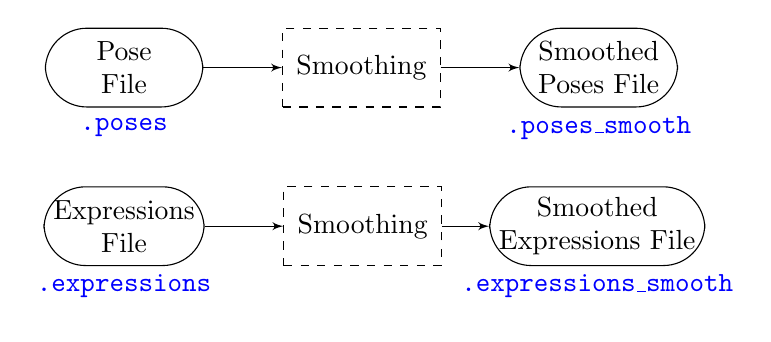
\begin{tikzpicture}[>=latex']
        \tikzset{block/.style= {draw, rectangle, align=center,minimum width=2cm,minimum height=1cm},
        dblock/.style= {draw=black,dashed,  align=center,minimum width=2cm,minimum height=1cm},
        int/.style={minimum size=2em,font=\ttfamily,text=blue},
        rblock/.style={draw, shape=rectangle,rounded corners=1.5em,align=center,minimum width=2cm,minimum height=1cm},
        input/.style={ % requires library shapes.geometric
        draw,
        trapezium,
        trapezium left angle=60,
        trapezium right angle=120,
        minimum width=2cm,
        align=center,
        minimum height=1cm
    },
        }
        \node [rblock]  (pose) {Pose\\File};
        \node [dblock, right=1cm of pose] (smoothp) {Smoothing};
        \node [int, below=-0.1cm of pose] (pose_ext) {.poses};
        \node [rblock, right=1cm of smoothp] (poses) {Smoothed \\Poses File};
        \node [int, below=-0.1cm of poses] (poses_ext) {.poses\_smooth};
        \node [rblock, below=1cm of pose]  (exp) {Expressions\\File};
        \node [int, below=-0.1cm of exp] (exp_ext) {.expressions};
        \node [dblock, right=1cm of exp] (smoothe) {Smoothing};
        \node [rblock, right=0.6cm of smoothe] (exps) {Smoothed\\Expressions File};
        \node [int, below=-0.1cm of exps] (exps_ext) {.expressions\_smooth};
%%% paths
        \path[draw,->] (pose) edge (smoothp)
                    (smoothp) edge (poses)
                    (exp) edge (smoothe)
                    (smoothe) edge (exps)
                    ;
    \end{tikzpicture}
    
\end{document}